\documentclass[10pt]{beamer}

\usepackage{listings}
\usepackage{tabularx}
\usepackage{multirow}
\usepackage{tikz}
\DeclareMathOperator{\Ima}{Im}
\usetikzlibrary{automata,positioning}

\usecolortheme{seagull}
\useoutertheme{infolines}
\usefonttheme[onlymath]{serif}

\title{Creating a Robust AspectMATLAB Compiler}
\author{Hongji Chen}
\date[September 1, 2016]{UCORE'16}

\begin{document}

\frame{\maketitle}

\begin{frame}[fragile]
\frametitle{Aspect Oriented Programming in Java (AspectJ)}
\begin{block}{Pointcuts}
A pointcut is a program element that picks out join points and exposes data
from the execution context of those join points. \cite{aspectjOnlinePointcut}

\begin{lstlisting}[basicstyle=\small, language=Java]
pointcut pCall() : call (* *.*(..))      // all function calls
pointcut pExec() : execution (* *.*(..)) // all function execs
pointcut pComp() : pCall() || pExec()    // both call and execs
\end{lstlisting}

\end{block}

\begin{block}{Pointcut Advice}
Advice defines crosscutting behavior. It is defined in terms of pointcuts. The
code of a piece of advice runs at every join point picked out by its pointcut. 
\cite{aspectjOnlineAdvice}

\begin{lstlisting}[basicstyle=\small, language=Java]
before() : pComp() {
    /* do something */
}
\end{lstlisting}
\end{block}
\end{frame}

\begin{frame}
\frametitle{Aspect Oriented Programming in Java (AspectJ)}
\begin{columns}
    \begin{column}[T]{0.5\textwidth}
    \textbf{Aspect File}
    \lstinputlisting[basicstyle=\tiny, language=Java]{DemoAspect.java}  
    \end{column}
    \begin{column}[T]{0.5\textwidth}
    \textbf{Target File}
    \lstinputlisting[basicstyle=\tiny, language=Java]{DemoTarget.java}  
    \end{column}
\end{columns}
\pause
\lstinputlisting[basicstyle=\tiny, language=Java]{DemoOut.out}    
 
\end{frame}

\begin{frame}
\frametitle{Aspect MATLAB Programming in MATLAB}
\framesubtitle{Previous Work}
\begin{itemize}
    \item Toheed Aslam's AspectMATLAB Compiler \cite{AspectMATLABpaper}
    \item Andrew Bodzay's AspcetMATLAB++ Compiler \cite{AspectMATLABPPpaper}
    \item McSAF Framework \cite{McSAF}, and Kind Analysis \cite{KindAnalysis}
    \item Samuel Suffos's Parser \cite{McLabParser}
\end{itemize}
\end{frame}

\begin{frame}
\frametitle{Aspect MATLAB Programming in MATLAB}
\begin{itemize}
    \item Pointcuts $\Rightarrow$ Patterns
    \item Pointcut Advice $\Rightarrow$ Actions
\end{itemize}
\end{frame}

\begin{frame}
\frametitle{Aspect MATLAB Programming in MATLAB}
\framesubtitle{Patterns and Actions}
\textbf{Patterns}
\begin{columns}
    \begin{column}[T]{0.5\textwidth}
        \begin{description}
            \item [Annotate]       annotation comment
            \item [Call]           subroutine call
            \item [Execution]      subroutine execution
            \item [Get]            variable read
            \item [Loop]           for-loop or while-loop
            \item [LoopHead]       loop initialization
            \item [LoopBody]       loop execution body
        \end{description}    
    \end{column}
    \begin{column}[T]{0.5\textwidth}
        \begin{description}
            \item [MainExecution]  entry point
            \item [Operator]       MATLAB matrix/array operation
            \item [Set]            variable write
            \item [Dimension]      restrict search by shape
            \item [IsType]         restrict search by type
            \item [Within]         restrict search by scope
        \end{description}    
    \end{column}
\end{columns}

\textbf{Actions}
\begin{description}
    \item [Before]  Action will be executed before the captured join point
    \item [After]   Action will be executed after the captured join point
    \item [Around]  Action will be executed instead of the captured join point
\end{description}
\end{frame}

\begin{frame}
\frametitle{Aspect MATLAB Programming in MATLAB}
\framesubtitle{Improvements and Contributions}
\begin{itemize}
    \item Use of More Robust Front-end
    \item Clear Grammar
    \item Semantic Validation
    \item More Robust Transforming Strategy
    \item Extended Argument Matching
\end{itemize}
\end{frame}

\begin{frame}[fragile]
\frametitle{Improvement on Grammar}
\textbf{Extended Get and Set Pattern} more clear pattern
\begin{lstlisting}[basicstyle=\small, language=MATLAB]
get(goo) & dimension([1,1]) & istype(logical)
set(*) & dimension([3,3,..]) & istype(double)
\end{lstlisting}
$\Rightarrow$
\begin{lstlisting}[basicstyle=\small, language=MATLAB]
get(goo : [1,1]logical)
set(* : [3,3,..]double)
\end{lstlisting}

\textbf{Enhanced Usage of Wildcards} allow wildcard to appear at any position
within argument list
\begin{lstlisting}[basicstyle=\small, language=MATLAB]
dimension([3,..,4])
\end{lstlisting}

\textbf{Extended Call and Execution Pattern} restrict matching according to
shape and type of arguments and return values.
\begin{lstlisting}[basicstyle=\small, language=MATLAB]
call(foo([1,1]function_handle, *, [..]double) : [1,3]logical)
\end{lstlisting}
\end{frame}

\begin{frame}[fragile]
\frametitle{Semantic Validation}
\textbf{Semantic Invalid Pattern and Action} may lead to unpredictable result
during AST transformation and weaving.
\begin{lstlisting}[basicstyle=\small, language=MATLAB]
% unbounded 'within pattern'
a1 : before within(function, foo) : ()
% annotation has no type nor shape
a2 : before annotate(*(..)) & istype(logical) & dimension([3,3]) : ()
% or operator RHS unbounded
a3 : after loop(for : i) || within(script, demo.m) : ()
% cannot predict type and shape of return values without invoking
a4 : before call(foo(..) : [1,1]logical) : ()
% same as above, but more complicate
a5 : before (get(*) & call(*(..))) & istype(integer) : ()
% unclear pattern apply not operation to get pattern
a6 : before ~get(foo : double) : ()
\end{lstlisting}
\end{frame}

\begin{frame}
\frametitle{Semantic Validation}
\begin{itemize}
    \item Basic Pattern Classification (primitive pattern and modifier pattern)
    \item Pattern Type Analysis
    \item Logical Reduction (resolve modifier pattern on primitive pattern)
    \item Modifier Validation and Weaving Method Validation
\end{itemize}
\end{frame}

\begin{frame}
\frametitle{Semantic Validation}
\framesubtitle{Basic Pattern Classification}
\begin{block}{Primitive Pattern}
Primitive patterns are patterns with actual joint point within MATLAB
source code.
\end{block}

\begin{columns}
    \begin{column}{0.5\textwidth}
    \begin{itemize}
        \item Get/Set Pattern
        \item Call/Execution Pattern
        \item Loop/LoopHead/LoopBody Pattern
    \end{itemize}    
    \end{column}
    
    \begin{column}{0.5\textwidth}
    \begin{itemize}
        \item MainExecution Pattern
        \item Annotation Pattern
        \item Operator Pattern
    \end{itemize}
    \end{column}
\end{columns}


\begin{block}{Modifier Pattern}
Unlike primitive patterns, modifier patterns do not provide joint points for
action weaving, instead, it pose restriction on the primitive pattern which
they bound to.
\end{block}

\begin{columns}
    \begin{column}{0.5\textwidth}
    \begin{itemize}
        \item Dimension Pattern
        \item IsType Pattern
    \end{itemize}    
    \end{column}
    
    \begin{column}{0.5\textwidth}
    \begin{itemize}
        \item Scope Pattern
    \end{itemize}
    \end{column}
\end{columns}
\end{frame}

\begin{frame}[fragile]
\frametitle{Semantic Validation}
\framesubtitle{Pattern Type Analysis}
\begin{columns}
    \begin{column}{0.5\textwidth}
    \textbf{And Compound Pattern}
    
    (Primitive $\land$ Primitive) $\rightarrow$ Primitive                    \\
    (Primitive $\land$ Modifier)  $\rightarrow$ Primitive                    \\
        \emph{\quad The Modifier pattern is bounded towards the primitive
    pattern and remove from further analysis.}                               \\
    (Modifier  $\land$ Primitive) $\rightarrow$ Primitive                    \\
    (Modifier  $\land$ Modifier)  $\rightarrow$ Modifier
    
    \end{column}
    \begin{column}{0.5\textwidth}
    \textbf{Or Compound Pattern}
    
    (Primitive $\lor$  Primitive) $\rightarrow$ Primitive                    \\
    (Primitive $\lor$  Modifier)  $\rightarrow$ Invalid                      \\
        \emph{\quad Cannot resolve right hand side modifier pattern to a
    primitive pattern, thus the modifier pattern is unbounded.}              \\
    (Modifier  $\lor$  Primitive) $\rightarrow$ Invalid                      \\
    (Modifier  $\lor$  Modifier)  $\rightarrow$ Modifier
    \end{column}
\end{columns}

\textbf{Not Compound Pattern}                                                \\
$\neg$ Primitive $\rightarrow$ Invalid                                       \\
\emph{\quad Ambiguous Pattern}                                               \\
$\neg$ Modifier  $\rightarrow$ Modifier                                      
\end{frame}

\begin{frame}[fragile]
\frametitle{Semantic Validation}
\framesubtitle{Pattern Simplification}
Simplify pattern using logical equivalence, moving modifier pattern towards
its bounded primitive pattern.

\begin{lstlisting}[basicstyle=\small, language=MATLAB]
(get(*) & call(*(..))) & ~(istype(integer) & istype(logical))
\end{lstlisting}
$\neg (A \land B) \equiv \neg A \lor \neg B$                                 \\
$\Rightarrow$
\begin{lstlisting}[basicstyle=\small, language=MATLAB]
(get(*) & call(*(..))) & (~istype(integer) | ~istype(logical))
\end{lstlisting}
$A \land (B \lor C) \equiv (A \land B) \lor (A \land C)$                     \\
$\Rightarrow$
\begin{lstlisting}[basicstyle=\small, language=MATLAB]
(get(*) & (~istype(integer) | ~istype(logical))) & 
    (call(*(..)) & (~istype(integer) | ~istype(logical)))
\end{lstlisting}

\end{frame}

\begin{frame}[fragile]
\frametitle{Semantic Validation}
\framesubtitle{Modifier Validation and Weaving Method Validation}
\begin{table}[]
\centering
\begin{tabular}{c|ccc|ccc|c}
\multirow{2}{*}{Pattern} & \multicolumn{3}{c|}{Dimension}             & \multicolumn{3}{c|}{IsType}                & \multirow{2}{*}{Scope} \\
                         & Before       & After        & Around       & Before       & After        & Around       &                        \\ \hline
Get/Set                  & $\checkmark$ & $\checkmark$ & $\checkmark$ & $\checkmark$ & $\checkmark$ & $\checkmark$ & $\checkmark$           \\
Call/Exec                & $\times$     & $\checkmark$ & $\times$     & $\times$     & $\checkmark$ & $\times$     & $\checkmark$           \\
Annotation               & $\times$     & $\times$     & $\times$     & $\times$     & $\times$     & $\times$     & $\checkmark$           \\
Loops                    & $\times$     & $\times$     & $\times$     & $\times$     & $\times$     & $\times$     & $\checkmark$           \\
MainExec                 & $\times$     & $\times$     & $\times$     & $\times$     & $\times$     & $\times$     & $\times$               \\
Operator                 & $\times$     & $\checkmark$ & $\times$     & $\times$     & $\checkmark$ & $\times$     & $\checkmark$          
\end{tabular}
\end{table}

\begin{lstlisting}[basicstyle=\small, language=MATLAB]
a5 : before (get(*) & call(*(..))) & istype(integer) : ()
\end{lstlisting}
$\Rightarrow$
\begin{lstlisting}[basicstyle=\small, language=MATLAB]
a5 : before (get(*) & (~istype(integer) | ~istype(logical))) & 
            (call(*(..)) & (~istype(integer) | ~istype(logical))) : ()
\end{lstlisting}
$\Rightarrow$
\textbf{Reject}
\end{frame}

\begin{frame}
\frametitle{More Robust Transforming Strategy}
\begin{itemize}
    \item Comma Separated List Handling 
    \item End Expression Resolve
    \item Set Pattern New Variable Capture
    \item $\dots$
\end{itemize}
\end{frame}

\begin{frame}[fragile]
\frametitle{More Robust Transforming Strategy}
\framesubtitle{Comma Separated List Handling}
\begin{lstlisting}[basicstyle=\small, language=MATLAB]
foo(c{:}, m(:).f, p);
\end{lstlisting}
with pattern
\begin{lstlisting}[basicstyle=\small, language=MATLAB]
get(*) | call(*(..))
\end{lstlisting}

\textbf{Current AspectMATLAB}
\begin{lstlisting}[basicstyle=\small, language=MATLAB]
AM_VAR_1 = c{:};
AM_VAR_2 = m(:).f;
AM_VAR_3 = p;
AM_VAR_4 = foo(AM_VAR_1, AM_VAR_2, AM_VAR_3);
\end{lstlisting}
$\Rightarrow$
\begin{lstlisting}[basicstyle=\small, language=MATLAB]
AM_VAR_1 = {c{:}};
AM_VAR_2 = {m(:).f};
AM_VAR_3 = p;
AM_VAR_4 = foo(AM_VAR_1{:}, AM_VAR_2{:}, AM_VAR_3);
\end{lstlisting}
\end{frame}

\begin{frame}[fragile]
\frametitle{More Robust Transforming Strategy}
\framesubtitle{End Expression Resolve}
\begin{lstlisting}[basicstyle=\small, language=MATLAB]
m(p1, end, c{:}, :)
\end{lstlisting}
with pattern
\begin{lstlisting}[basicstyle=\small, language=MATLAB]
get(*)
\end{lstlisting}

\textbf{Current AspectMATLAB}

Ignored

$\Rightarrow$

\begin{lstlisting}[basicstyle=\small, language=MATLAB]
AM_VAR_1 = p1;
AM_VAR_2 = {c{1:builtin('end', c, 1, 1)}};
AM_VAR_3 = sum([1, 1, length(AM_VAR_2), 1]);
AM_VAR_4 = m(
             AM_VAR_1, 
             builtin('end', m, sum([1, 1]), AM_VAR_3),
             AM_VAR_3,
             1:builtin('end', m, 
                       sum([1, 1, length(AM_VAR_2), 1]), 
                       AM_VAR_3)
            );
\end{lstlisting}
\end{frame}

\begin{frame}[fragile]
\frametitle{More Robust Transforming Strategy}
\framesubtitle{Set Pattern New Variable Capture}
\begin{lstlisting}[basicstyle=\small, language=MATLAB]
[var1, c{1:2}] = foo();
\end{lstlisting}
with pattern
\begin{lstlisting}[basicstyle=\small, language=MATLAB]
set(*)
\end{lstlisting}
\textbf{Current AspectMATLAB}
\begin{lstlisting}[basicstyle=\small, language=MATLAB]
[var1, c{1:2}] = foo();           % both new value as foo()
\end{lstlisting}
$\Rightarrow$
\begin{lstlisting}[basicstyle=\small, language=MATLAB]
if exist('var1', 'var')
    AM_VAR_1 = var1;
end
if exist('c', 'var')
    AM_VAR_2 = c;
end
[AM_VAR_1, AM_VAR_2{1:2}] = foo();
[var1] = deal(AM_VAR_1);           % new value as AM_VAR_1
[c{1:2}] = deal(AM_VAR_2{1:2});    % new value as AM_VAR_2
\end{lstlisting}
\end{frame}

\begin{frame}[fragile]
\frametitle{Extended Argument Matching}
\textbf{Current AspectMATLAB}
\begin{lstlisting}[basicstyle=\small, language=MATLAB]
call(foo(*,..))
\end{lstlisting}
\begin{itemize}
    \item Matching according to the number of input arguments
    \item dots wildcard only allow to appear at the end of the pattern list
\end{itemize}

\pause

\begin{lstlisting}[basicstyle=\small, language=MATLAB]
call(foo(*, .., [1,*,..,2,3]double) : [..]logical, [2,2]*)
\end{lstlisting}
\begin{itemize}
    \item Matching according to both input and output (restriction applied)
    \item Dots wildcards can appear at any part in the signature list
    \item Shape and Type information matching
\end{itemize}    
\end{frame}

\begin{frame}
\frametitle{Extended Argument Matching}
\begin{itemize}
    \item Collect Alphabet
    \item Building nondeterministic finite automaton for shape patterns
    \item Convert nondeterministic finite automaton into deterministic
          finite automaton
    \item Emit matcher function
\end{itemize}
\end{frame}

\begin{frame}[fragile]
\frametitle{Extended Argument Matching}
\framesubtitle{Collect Alphabet}
\textbf{Why?} We need a finite alphabet to built NFA and DFA. But, in MATLAB,
any valid identifier can be a valid type name, and dimension can be a list of
any positive integers.

Trivial solution. $\times$

\pause

Construct alphabet $\Sigma$ as follow:
\begin{itemize}
    \item $\epsilon \in \Sigma$
    \item if symbol $s$ appears in signature, then $s \in \Sigma$
    \item let $\sigma$ be a special symbol, denoting any other symbol that
          don't appear in the signature
\end{itemize}
Then the alphabet $\Sigma$ is a finite set, as we have a finite signature.

\pause
\begin{lstlisting}[basicstyle=\small, language=MATLAB]
call(foo(*, .., [1,*,..,2,3]double) : [..]logical, [2,2]*)
\end{lstlisting}
$\Sigma_{shape} = \lbrace \epsilon_{shape}, 1, 2, 3, \sigma_{shape} \rbrace$ \\
$\Sigma_{type} = \lbrace \epsilon_{type}, \text{double},
                         \text{logical}, \sigma_{type} \rbrace$              
\end{frame}

\begin{frame}[fragile]
\frametitle{Extended Argument Matching}
\framesubtitle{Building nondeterministic finite automaton for shape patterns}
\textbf{Pattern with only shape matching}
\begin{lstlisting}[basicstyle=\small, language=MATLAB]
dimension([1, *, .., 2, 3])
\end{lstlisting}
Alphabet : $\Sigma_{shape} = \lbrace \epsilon, 1, 2, 3, \sigma \rbrace$
\begin{tikzpicture}[shorten >=1pt,node distance=1.3cm,on grid,auto] 
    \node[state, initial]   (0)               {$0$};
    \node[state]            (1) [right of=0]  {$1$};
    \node[state]            (2) [right of=1]  {$2$};
    \node[state]            (3) [right of=2]  {$3$};
    \node[state]            (4) [right of=3]  {$4$};
    \node[state]            (5) [right of=4]  {$5$};
    \node[state]            (6) [right of=5]  {$6$};
    \node[state, accepting] (7) [right of=6]  {$7$};
    \path[->]
    (0)      edge node                 {$1$}                      (1)
    (1)      edge [bend left]node      {$1,2,3,\sigma$}           (2)
    (2)      edge node                 {$\epsilon$}               (3)
    (3)      edge [bend left]node      {$1,2,3,\sigma,\epsilon$}  (4)
    (4)      edge node                 {$\epsilon$}               (5)
    (5)      edge node                 {$2$}                      (6)
             edge [bend left]node      {$\epsilon$}               (2)
    (6)      edge node                 {$3$}                      (7);
\end{tikzpicture}
\textbf{Pattern with only type matching}
\begin{lstlisting}[basicstyle=\small, language=MATLAB]
call(foo(logical, *, .., double))
\end{lstlisting}
Alphabet : $\Sigma_{type} = \lbrace \epsilon, \text{logical}, 
                                    \text{double}, \sigma \rbrace$

\begin{tikzpicture}[shorten >=1pt,node distance=1.5cm,on grid,auto] 
    \node[state, initial]   (0)               {$0$};
    \node[state]            (1) [right of=0]  {$1$};
    \node[state]            (2) [right of=1]  {$2$};
    \node[state]            (3) [right of=2]  {$3$};
    \node[state]            (4) [right of=3]  {$4$};
    \node[state]            (5) [right of=4]  {$5$};
    \node[state, accepting] (6) [right of=5]  {$6$};
    \path[->] 
    (0)     edge [bend left]node     {$\text{logical}$}                    (1)
    (1)     edge [bend left]node     {$\Sigma_{type} \setminus \lbrace
                                       \epsilon \rbrace$}                  (2)
    (2)     edge node                {$\epsilon$}                          (3)
    (3)     edge node                {$\Sigma_{type}$}                     (4)
    (4)     edge node                {$\epsilon$}                          (5)
    (5)     edge [bend left]node     {$\text{double}$}                     (6)
            edge [bend left]node     {$\epsilon$}                          (2);
\end{tikzpicture}
\end{frame}

\begin{frame}[fragile]
\frametitle{Extended Argument Matching}
\framesubtitle{Convert NFAs into DFAs}
\textbf{Using subset construction method}

\begin{columns}
\begin{column}[T]{0.5\textwidth}
\begin{lstlisting}[basicstyle=\small, language=MATLAB]
dimension([1, *, .., 2, 3])
\end{lstlisting}
Alphabet Map : $\lbrace 1 = 1, 2 = 2, 3 = 3, \sigma = 4 \rbrace$             \\
Matrix representation of DFA in MATLAB:
\begin{lstlisting}[basicstyle=\small, language=MATLAB]
AM_FUNC_8 = [2, 6, 6, 6; 
             3, 3, 3, 3; 
             3, 4, 3, 3; 
             3, 4, 5, 3; 
             3, 4, 3, 3; 
             6, 6, 6, 6];
\end{lstlisting}
\end{column}
\begin{column}[T]{0.5\textwidth}
\begin{lstlisting}[basicstyle=\small, language=MATLAB]
call(foo(logical, *, .., double))
\end{lstlisting}
Alphabet Map : $\lbrace \text{logical} = 1, \text{double} = 2, 
                        \sigma = 3                              \rbrace$     \\
                        Matrix representation of DFA in MATLAB:
\begin{lstlisting}[basicstyle=\small, language=MATLAB]
AM_FUNC_4 = [2, 5, 5; 
             3, 3, 3; 
             3, 4, 3; 
             3, 4, 3; 
             5, 5, 5];
\end{lstlisting}
\end{column}
\end{columns}
\end{frame}

\begin{frame}[fragile]
\frametitle{Extended Argument Matching}
\framesubtitle{Emit matcher function}
\begin{lstlisting}[basicstyle=\small, language=MATLAB]
call(foo(logical, *, .., double))
\end{lstlisting}
$\Rightarrow$
\begin{lstlisting}[basicstyle=\tiny, language=MATLAB]
function [AM_FUNC_3] = AM_VAR_1(AM_FUNC_2)
  AM_FUNC_4 = [2, 5, 5; 3, 3, 3; 3, 4, 3; 3, 4, 3; 5, 5, 5];
  AM_FUNC_5 = 1;
  for AM_FUNC_6 = (1 : length(AM_FUNC_2))
    AM_FUNC_5 = AM_FUNC_4(AM_FUNC_5, AM_VAR_0(AM_FUNC_2{AM_FUNC_6}));
  end
  AM_FUNC_7 = [4];
  for AM_FUNC_8 = (1 : length(AM_FUNC_7))
    if (AM_FUNC_5 == AM_FUNC_7(AM_FUNC_8))
      AM_FUNC_3 = true;
      return
    end
  end
  AM_FUNC_3 = false;
  return
  function [AM_FUNC_1] = AM_VAR_0(AM_FUNC_0)
    if isa(AM_FUNC_0, 'double')
      AM_FUNC_1 = 2;
    elseif isa(AM_FUNC_0, 'logical')
      AM_FUNC_1 = 1;
    else 
      AM_FUNC_1 = 3;
    end
  end
end
\end{lstlisting}
\end{frame}

\begin{frame}[fragile]
\frametitle{Extended Argument Matching}
\framesubtitle{More complicate pattern}
\begin{lstlisting}[basicstyle=\small, language=MATLAB]
call(foo([1, 2, .., 3]logical, *, .., [1, .., 2, 3]logical))
pattern1 = [1, 2, .., 3]logical
pattern2 = [1, .., 2, 3]logical
\end{lstlisting}
Previous solution won't work, as alphabet is not a surjective map from
variables to symbol code.

\textbf{Alternative solution:}
let $S_{pattern1}$ denotes the set of variable matching to pattern1, 
$S_{pattern2}$ denotes the set of variable matching to pattern2, and $S$
denotes the set of all possible input variables. Then alphabet $A =
\lbrace \epsilon, s_1, s_2, s_3, \sigma \rbrace$, with following map $\tau : S
\rightarrow A$ is a suitable candidate for NFA/DFA construction, and
$A \supseteq \Ima \tau$ is a finite set with at most $2^{\vert \sharp
\text{patterns}
\vert} + 1$ symbols.
\begin{equation*}
    \tau(x) = 
         \begin{cases}
            \epsilon       &\epsilon \text{-transition}                      \\
            s_1            &x \in S_{pattern1} \setminus S_{pattern2}        \\
            s_2            &x \in S_{pattern2} \setminus S_{pattern1}        \\
            s_3            &x \in S_{pattern1} \cap S_{pattern2}             \\
            \sigma         &x \in (S_{pattern1} \cup S_{pattern2})^{\mathsf{c}}
        \end{cases}
\end{equation*}

\end{frame}

\begin{frame}[fragile]
\frametitle{Extended Argument Matching}
\framesubtitle{Analysis on performance}
\textbf{If a pattern has $m$ signature with $k$ dots wildcards.}

The modified NFA/DFA method use $m * (m-k)$ times shape and type checking.   \\
The for-loop based method use $k^{m-k} + k$ times shape and type checking.   \\
\begin{columns}
\begin{column}[T]{0.5\textwidth}
Plot under $m = 10$,                                                         \\
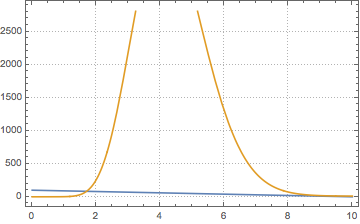
\includegraphics[scale=0.4]{plot}    
\end{column}
\begin{column}[T]{0.5\textwidth}
Plot under $m = 5$,                                                          \\
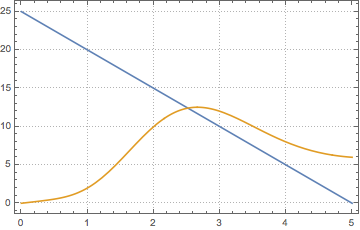
\includegraphics[scale=0.4]{plot_small}    
\end{column}
\end{columns}
$\Rightarrow$                                                                \\
Implemented as for-loop based method for patterns with few dots wildcard
(1-2), NFA/DFA method for other scenario.
\end{frame}

\begin{frame}[fragile]
\frametitle{Extended Argument Matching}
\framesubtitle{Using matcher function}
\textbf{Input argument matching:}
\begin{lstlisting}[basicstyle=\small, language=MATLAB]
foo(var1, var2(:).f, var3{:})
\end{lstlisting} 
$\Rightarrow$
\begin{lstlisting}[basicstyle=\small, language=MATLAB]
AM_VAR_1 = {var1, var2(:), var{:}};
AM_MATCH_RESULT(1) = matcher1(AM_VAR_1);
AM_MATCH_RESULT(2) = matcher2(AM_VAR_2);
% ...
foo(AM_VAR_1{:})
\end{lstlisting}

\textbf{Output argument matching:}
\begin{lstlisting}[basicstyle=\small, language=MATLAB]
foo(var1, var2(:).f, var3{:})
\end{lstlisting} 
$\Rightarrow$
\begin{lstlisting}[basicstyle=\small, language=MATLAB]
% callWithMatcher is a MEX implemented subroutine using C
AM_VAR_1 = {var1, var2(:), var{:}};
[AM_MATCH_RESULT, ...] = callWithMatcher(
                             @foo, AM_VAR_1, 
                             @matcher1, @matcher2, ...
                         );
\end{lstlisting}
\end{frame}

\bibliographystyle{plainurl}
\bibliography{reference}
\end{document}